% !TEX program = xelatex
%%%%%%%%%%%%%%%%%%%%%%%%

\documentclass[11pt,aspectratio=169]{beamer} % 11pt is default
\usetheme{metropolis} % [progressbar=frametitle]
\setbeamercolor{background canvas}{bg=white}
\setbeamertemplate{caption}{\insertcaption} 
\setbeamersize{text margin left=2em,text margin right=2em}
\setbeamertemplate{frame footer}{\vspace{-5pt}}

\usepackage[round]{natbib}
\usepackage{amsmath}
\usepackage{mathtools}
\usepackage[group-minimum-digits=4,group-separator={,}]{siunitx}
\usepackage{graphicx}
\usepackage{wrapfig}
\usepackage{multimedia}

\usepackage{tikz}
\usetikzlibrary{backgrounds}
\usetikzlibrary{arrows,shapes}
\usetikzlibrary{tikzmark}
\usetikzlibrary{calc}
\usepackage[dvipsnames]{xcolor}

\usepackage[skins,theorems]{tcolorbox}
\usepackage{pdfpages}
\usepackage{colortbl}
\usepackage{changepage}
\usepackage{booktabs}
\usepackage{makecell}
\usepackage{setspace}
\usepackage{algorithm}
\usepackage[noend]{algpseudocode}
\usepackage{subcaption}
\usepackage[framemethod=TikZ]{mdframed}
\usepackage{xspace}

\usepackage{annotate-equations}

% Shortcut for beamer frames
\newcommand{\bframe}[2][c]{\begin{frame}[#1]{#2}}
\newcommand{\eframe}{\end{frame}} % \eframe causes problems for some reason

% Shortcut for bold text
\newcommand{\fat}[1]{\textbf{#1}}

% Boxing items on slide
\newcommand{\Cboxed}[2]{\colorlet{currentcolor}{.}{\color{#1}\fbox{\color{currentcolor}#2}}} %create coloured box around equation

% checkmark and xmark
\usepackage{pifont}
\newcommand{\cmark}{\ding{51}}%
\newcommand{\xmark}{\ding{55}}%

% Highlighting text in orange
\newcommand{\e}[1]{\alert{#1}}

% Underline
\newcommand{\uline}[1]{\underline{#1}}

% Include figure
\newcommand{\imgw}[2]{\includegraphics[width=#2\textwidth]{#1}} % \imgw{file}{height-scale}
\newcommand{\imgh}[2]{\includegraphics[height=#2\textheight]{#1}} % \imgh{file}{width-scale}

% Shortcut for latex commands
\newcommand{\blist}{\vspace{-3pt}\begin{list}{\raisebox{1pt}{\small$\bullet$}}{\leftmargin=13pt\itemsep=4pt}}
\newcommand{\blisttab}{\vspace{5pt}\blist}
\newcommand{\elisttab}{\end{list}}
\newcommand{\listtab}{\\[3pt] $\Rightarrow$ }
\newcommand{\elist}{\end{list}\vspace{5pt}}
\newcommand{\bblock}[1]{\metroset{block=fill}\begin{block}{#1}}
\newcommand{\eblock}{\end{block}}
\newcommand{\bmath}[1][0]{\begin{equation*}\hspace{#1em}}
\newcommand{\emath}{\end{equation*}}
\newcommand{\bcol}{\begin{columns}}
\newcommand{\col}[1]{\column{#1\textwidth}}
\newcommand{\tcol}[1]{\column[T]{#1\textwidth}}
\newcommand{\ecol}{\end{columns}}
\newcommand{\place}[4]{\begin{textblock}{#3}(#1,#2) #4 \end{textblock}} % \place{x}{y}{width}{text}
\newcommand{\placeframed}[4]{\place{#1}{#2}{#3}{\fbox{\parbox{#3em}{#4}}}}
\newcommand{\placeimg}[4]{\place{#1}{#2}{#3}{\imgw{#4}{1}}} % \placeimg{x}{y}{width}{file}
\newcommand{\videolink}[2]{\movie[externalviewer]{{\bf Video:} #1}{videos/#2}} % \videolink{title}{file}
\newcommand{\btab}[1]{\begin{tabular}{#1}}
\newcommand{\etab}{\end{tabular}}
\newcommand{\balgo}[2][1.3]{{#2:} \\[5pt] \begin{algorithmic}[1] \linespread{#1}\selectfont}
\newcommand{\ealgo}{\end{algorithmic}}
\renewcommand{\algorithmicloop}{\textbf{repeat:}}
\newcommand{\cred}{\cellcolor{red!25}}
\newcommand{\cgreen}{\cellcolor{green!25}}

% Shortcut for commonly used math symbols
\newcommand{\condpr}[2]{\text{Pr}\hspace{-1pt}\left\{ #1 \ \mid \ #2 \right\}}
\newcommand{\exarg}[2]{\mathbb{E}_{#1}\hspace{-2pt}\left[ #2 \right]}
\newcommand{\exnoarg}[1]{\mathbb{E}_{#1}}
\NewDocumentCommand\ex{ m g }{
	\IfNoValueTF{#2}{\exnoarg{#1}}{\exarg{#1}{#2}}
}
\newcommand{\der}[2]{\frac{\partial #1}{\partial #2}}
\newcommand{\stats}{\mathcal{S}}
\newcommand{\acts}{\mathcal{A}}
\newcommand{\rews}{\mathcal{R}}
\newcommand{\eps}{\mathcal{E}}
\newcommand{\ver}{\,\vert\,}
\newcommand{\vhat}{\hat{v}}
\newcommand{\qhat}{\hat{q}}
% \newcommand{\para}{\textbf{w}}
\newcommand{\feats}{\textbf{x}}
\newcommand{\elig}{\textbf{z}}
\newcommand{\gradient}{\nabla}
\newcommand{\outline}{Lecture Outline}
\newcommand{\reading}{Reading}
\newcommand{\h}[1]{\emph{#1}}

\emph
% \newcommand{\lindex}[1]{%
% 	\lowercase{\def\temp{#1}%
% 	\expandafter\index\expandafter{\temp}%
% }

\newcommand{\indx}[1]{\index{#1}}
\newcommand{\hind}[1]{\h{#1}\lindex{#1}}

% Set of real numbers
\newcommand{\R}{\mathbb{R}}
% Proportional to
% Transpose of a vector x
\newcommand{\vectranspose}[1]{#1^\top}
% Transpose of a matrix X
\newcommand{\mattranspose}[1]{#1^\top}
% Probability
\newcommand{\pr}{\text{Pr}}
% Conditional probability of x given y
\newcommand{\cpr}[2]{\pr( #1 \mid #2 )}
% x sampled according to probability distribution p
\newcommand{\sampled}[2]{#1 \sim #2}
% Assign value y to variable x
\newcommand{\assign}[2]{#1 \gets #2}
% Training data set
\newcommand{\data}{\mathcal{D}}
% Concatenation of inputs a, b, c, ...
\newcommand{\con}[1]{\langle #1 \rangle}
% array with bracket
\newcommand{\bra}[2]{\left[ \begin{array}{#1} #2 \end{array} \right]}
% Indicator function: returns 1 if x is true, otherwise returns 0
\newcommand{\ind}[1]{[#1]_1}

% common way of referring to places
\newcommand{\seehere}[1]{(\cref{#1})}

% shortcut text commands
\newcommand{\rl}{RL\xspace}
\newcommand{\marl}{MARL\xspace}
\newcommand{\ctde}{CTDE\xspace}
\newcommand{\sa}{single-agent\xspace}
\newcommand{\ma}{multi-agent\xspace}
\newcommand{\Ma}{Multi-agent\xspace}
\newcommand{\mas}{multi-agent system\xspace}
\newcommand{\stat}{stationarity\xspace}
\newcommand{\nonstat}{non-stationarity\xspace}
\newcommand{\pg}{policy gradient\xspace}
\newcommand{\vb}{value-based\xspace}
\newcommand{\pbt}{population-based training\xspace}
\newcommand{\psro}{policy space response oracles\xspace}
\newcommand{\Psro}{Policy space response oracles\xspace}
\newcommand{\sct}{\emph{StarCraft~II}\xspace}
\newcommand{\as}{AlphaStar\xspace}
\newcommand{\az}{AlphaZero\xspace}
\newcommand{\lbf}{level-based foraging\xspace}
\newcommand{\Lbf}{Level-based foraging\xspace}
\newcommand{\nfg}{normal-form game\xspace}
\newcommand{\nfgs}{normal-form games\xspace}
\newcommand{\Nfg}{Normal-form game\xspace}
\newcommand{\Nfgs}{Normal-form games\xspace}
\newcommand{\rps}{Rock-Paper-Scissors\xspace}
\newcommand{\pd}{Prisoner's Dilemma\xspace}
\newcommand{\survey}[4]{\noindent #1 (#4). ``#2.'' In: {\it #3}. \\}
\newcommand{\nashprob}{\textsc{Nash}\xspace}
\newcommand{\eol}{\textsc{End-of-Line}\xspace}
\newcommand{\ul}[1]{\underline{#1}}
\newcommand\norm[1]{\lVert#1\rVert}
\newcommand{\qlearn}{Q-learning\xspace}
\newcommand{\sarsa}{Sarsa\xspace}
\newcommand{\bayes}{Bayesian\xspace}
\newcommand{\bellman}{Bellman\xspace}
\newcommand{\markov}{Markov\xspace}
\newcommand{\pareto}{Pareto\xspace}
\newcommand{\boltzmann}{Boltzmann\xspace}
\newcommand{\mc}{Monte Carlo\xspace}
\newcommand{\nash}{Nash\xspace}
\newcommand{\ppad}{PPAD}
\newcommand{\dqn}{deep Q-networks\xspace}
\newcommand{\reinforce}{REINFORCE\xspace}
\newcommand{\qmix}{QMIX\xspace}
\newcommand{\qtran}{QTRAN\xspace}
\newcommand{\adam}{Adam\xspace}
\newcommand{\nret}{{$N$}-step returns\xspace}

% COMMANDS FOR COMMON NOTATION

% agent set
% state space
\newcommand{\St}{S}
\newcommand{\Stterm}{\bar{\St}}
% state
\newcommand{\st}{s}
\newcommand{\sth}{\hat{\st}}
% observation space
\newcommand{\Ob}{O}

% observation
\newcommand{\ob}{o}

% joint observation
\newcommand{\job}{o}
% action space
\newcommand{\Ac}{A}

% action
\newcommand{\ac}{a}
\newcommand{\ach}{\hat{\ac}}

% joint action
\newcommand{\jac}{a}
% reward
\newcommand{\rew}{r}
\newcommand{\rewh}{\hat{\rew}}
% centralised information
\newcommand{\ci}{z}

% initial state distribution

\newcommand{\instdist}{\mu}
% % state transition function

\newcommand{\Stf}{\mathcal{T}}
% % simulation/sampling model
\newcommand{\Stfsim}{\widehat{\Stf}}

% observation function
\newcommand{\Obf}{\mathcal{O}}

% reward function
\newcommand{\Rew}{\mathcal{R}}

% POLICIES, RETURNS, VALUES

% policy space
\newcommand{\Pol}{\Pi}

% policy
\newcommand{\pol}{\pi}
\newcommand{\poltil}{\tilde{\pol}}

% set of histories
\newcommand{\His}{H}
\newcommand{\Fhis}{\hat{\His}}
% history
\newcommand{\his}{h}

% full history
\newcommand{\fhis}{\hat{\his}}

% observation history extracted from full history
\newcommand{\obsext}{\sigma}

% discount factor
\newcommand{\dsc}{\gamma}

% return
\newcommand{\ret}{u}

% expected return for joint policy
\newcommand{\exret}{U}

% Agents
\newcommand{\Ag}{I}

% RL / MARL

% learning algorithm

\newcommand{\alg}{\mathbb{L}}

% empirical distribution/ average policy
\newcommand{\empdis}{\bar{\pol}}
\newcommand{\avgpol}{\bar{\pol}}
\newcommand{\agmod}{\hat{\pol}}
\newcommand{\Agmod}{\hat{\Pol}}
\newcommand{\agmodj}{agent model for agent $j$}

% best response
\newcommand{\br}{\textnormal{BR}}

% game value
\newcommand{\gval}{Value}

% value under agent model
\newcommand{\amval}{AV}

% regret
\newcommand{\regret}{Regret}
\newcommand{\avgreg}{\bar{R}}
% TD target
\newcommand{\target}{\mathcal{X}}
% step size (for gradient-based MARL in Chapter 5)
\newcommand{\step}{\kappa}


% DEEP LEARNING

% parameters
\newcommand{\para}{\theta}

% loss
\newcommand{\loss}{\mathcal{L}}
% batch
\newcommand{\batch}{\mathcal{B}}
\newcommand{\batchsize}{B}

% etnropy
\newcommand{\entropy}{\mathcal{H}}

% Create algorithm environment
\newcommand{\balg}[2]{
  \begin{algorithm}[H]
    \caption{#1}
    \label{alg:#2}
    \setstretch{1.1}
    \begin{algorithmic}[1]}

\newcommand{\ealg}{
    \end{algorithmic}
  \end{algorithm}}

% Argmin/ Argmax operators

\DeclareMathOperator*{\argmin}{arg\,min} 
\DeclareMathOperator*{\argmax}{arg\,max}

\makeatletter
\newenvironment{myitemize}{%
   \setlength{\topsep}{0pt}
   \setlength{\partopsep}{0pt}
   \renewcommand*{\@listi}{\leftmargin\leftmargini \parsep\z@ \topsep\z@ \itemsep\z@}
   \let\@listI\@listi
   \itemize
}{\enditemize}
\makeatother  

% define widebar for target parameters
\makeatletter
\newcommand*\rel@kern[1]{\kern#1\dimexpr\macc@kerna}
\newcommand*\widebar[1]{%
	\begingroup
	\def\mathaccent##1##2{%
		\rel@kern{0.8}%
		\overline{\rel@kern{-0.8}\macc@nucleus\rel@kern{0.2}}%
		\rel@kern{-0.2}%
	}%
	\macc@depth\@ne
	\let\math@bgroup\@empty \let\math@egroup\macc@set@skewchar
	\mathsurround\z@ \frozen@everymath{\mathgroup\macc@group\relax}%
	\macc@set@skewchar\relax
	\let\mathaccentV\macc@nested@a
	\macc@nested@a\relax111{#1}%
	\endgroup
}
\makeatother


% MATRIX GAMES

\newcolumntype{?}{!{\vrule width 1pt}}
\newcommand{\bhline}{\Xhline{1pt}}
\newcommand{\gametwo}[3]{
	\begin{tabular}{c?c|c}
		 & #1 \\
		\bhline
		#2    \\
		\hline
		#3    \\
	\end{tabular}
}
\newcommand{\gamethree}[4]{
	\begin{tabular}{c?c|c|c}
		 & #1 \\
		\bhline
		#2    \\
		\hline
		#3    \\
		\hline
		#4    \\
	\end{tabular}
}

\newcommand{\gamepd}{
    % \gametwo{C & D}{C & -1,-1 & -5,0}{D & 0,-5 & -3,-3}
	\begin{tabular}{c|c|c}
	& C & D \\
	\hline
	C & -1,-1 & -5,0 \\
	\hline
	D & 0,-5 & -3,-3
	\end{tabular}
}

\newcommand{\gamerps}{
    % \gamethree{R & P & S}{R & 0,0 & -1,1 & 1,-1}{P & 1,-1 & 0,0 & -1,1}{S & -1,1 & 1,-1 & 0,0}
	\begin{tabular}{c|c|c|c}
	& R & P & S \\
	\hline
	R & 0,0 & -1,1 & 1,-1 \\
	\hline
	P & 1,-1 & 0,0 & -1,1 \\
	\hline
	S & -1,1 & 1,-1 & 0,0
	\end{tabular}
}

\newcommand{\gamecoord}{
    % \gametwo{A & B}{A & 10 & 0}{B & 0 & 10}
	\begin{tabular}{c|c|c}
		& A & B \\
		\hline
		A & 10 & 0 \\
		\hline
		B & 0 & 10 \\
	\end{tabular}
}

\newcommand{\gamechicken}{
    % \gametwo{S & L}{S & 0,0 & 7,2}{L & 2,7 & 6,6}
	\begin{tabular}{c|c|c}
		& S & L \\
		\hline
		S & 0,0 & 7,2 \\
		\hline
		L & 2,7 & 6,6
	\end{tabular}
}

\newcommand{\gamestaghunt}{
    % \gametwo{S & H}{S & 4,4 & 0,3}{H & 3,0 & 2,2}
	\begin{tabular}{c|c|c}
		& S & H \\
		\hline
		S & 4,4 & 0,3 \\
		\hline
		H & 3,0 & 2,2
	\end{tabular}
}

\newcommand{\gamebattle}{
    \begin{tabular}{c|c|c}
    & A & B \\
    \hline
    A & 10,7 & 2,2 \\
    \hline
    B & 0,0 & 7,10
    \end{tabular}
}

\newcommand{\gameepsne}{
    % \gametwo{C & D}{A & 100,100 & 0,0}{B & 1,2 & 1,1}
	\begin{tabular}{c|c|c}
		& C & D \\
		\hline
		A & 100,100 & 0,0 \\
		\hline
		B & 1,2 & 1,1
	\end{tabular}
}

% Define colorboxes
\tcbset{
  % Defaults
  my box/main style/.style={},
  my box/title style/.style={},
  % Use the 'append' variants if you want to add to the defaults instead of
  % overriding them.
  my box/main/.style={/tcb/my box/main style/.style={#1}},
  my box/title/.style={/tcb/my box/title style/.style={#1}},
  my box/append main/.style={/tcb/my box/main style/.append style={#1}},
  my box/append title/.style={/tcb/my box/title style/.append style={#1}},
  %
  my box/.style={
    my box/.cd, #1,
    /tcb/.cd,
    enhanced,
    my box/main style,
    attach boxed title to top left={xshift=0.2cm, yshift=-0.2cm},
    top=10pt,
    boxed title style={
      outer arc=0pt,
      arc=0pt,
      top=3pt,
      bottom=3pt,
      my box/title style,
    },
  },
}

% define 'solutionbox' environment with coloured box
\newtcolorbox{solutionbox}[1][]{
  my box={
    main={colframe=green!40!gray!90, colback=green!20!gray!5},
    title={colback=green!40!gray!90},
  },
  title=Solution,
  #1,
}

\newtcolorbox{problembox}[1][]{
  my box={
    main={colframe=red!40!gray!90, colback=red!20!gray!5},
    title={colback=red!40!gray!90},
  },
  title=Problem,
  #1,
}

\newtcolorbox{notebox}[1][]{
  my box={
    main={colframe=orange!40!gray!80, colback=orange!20!gray!5},
    title={colback=orange!40!gray!80},
  },
  title=Note,
  #1,
}

\newtcolorbox{intuitionbox}[1][]{
  my box={
    main={colframe=blue!60!gray!80, colback=blue!20!gray!5},
    title={colback=blue!60!gray!80},
  },
  title=Intuition,
  #1,
}

\newtcolorbox{reminderbox}[1][]{
  my box={
    main={colframe=black!40!gray, colback=gray!10!white},
    title={colback=black!40!gray},
  },
  title=Reminder,
  #1,
}

\newtcolorbox{custombox}[2][]{
  my box={
    main={colframe=black!40!gray, colback=gray!10!white},
    title={colback=black!40!gray},
  },
  title={#2},
  #1,
}

% no title boxes
\newtcolorbox{greenbox}[1][]{
  my box={
    main={colframe=green!40!gray!90, colback=green!20!gray!5},
  },
  #1,
}
\newtcolorbox{redbox}[1][]{
  my box={
    main={colframe=red!40!gray!90, colback=red!20!gray!5},
  },
  #1,
}
\newtcolorbox{orangebox}[1][]{
  my box={
    main={colframe=orange!40!gray!80, colback=orange!20!gray!5},
  },
  #1,
}
\newtcolorbox{bluebox}[1][]{
  my box={
    main={colframe=blue!60!gray!80, colback=blue!20!gray!5},
  },
  #1,
}
\newtcolorbox{blackbox}[1][]{
  my box={
    main={colframe=black!55!black, colback=gray!5!white},
  },
  #1,
}


% Define intro slide command
\newcommand{\introslide}{
    \begin{frame}{MARL Book}
        \begin{columns}
            \begin{column}{0.5\textwidth}
            \begin{figure}
              \centering
              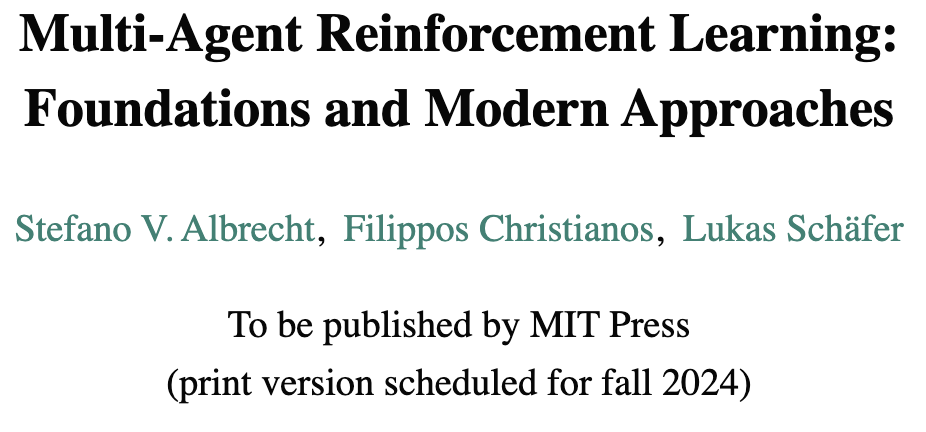
\includegraphics[width=\textwidth,height=.8\textheight,keepaspectratio]{images/1_MARL_book.png}
            
              \label{fig:enter-label}
            \end{figure}
          \end{column}
        
        \hspace{20pt}
            
          % Column for the text
            \begin{column}{0.45\textwidth}
	        \small

                This lecture is based on \textit{Multi-Agent Reinforcement Learning: Foundations and Modern Approaches} by Stefano V. Albrecht, Filippos Christianos and Lukas Sch\"afer
                
                \vspace{20pt}
                
                The book can be downloaded for free at \textcolor{blue}{\href{https://www.marl-book.com/}{www.marl-book.com}}.
            \end{column}
        
        \end{columns}
    \end{frame}
}

\newcommand{\leoslide}{
  \author{Stefano V. Albrecht, Filippos Christianos, Lukas Sch\"afer \\ Slides by: Leonard Hinckeldey}
}

\newcommand{\otherslide}{
  \author{Stefano V. Albrecht, Filippos Christianos, Lukas Sch\"afer}
}
	
\title{Multi-Agent Reinforcement Learning}
\date{}

\hypersetup{
  pdfsubject = {Multi-Agent Reinforcement Learning},
}

\otherslide

\subtitle{Multi-Agent Deep Reinforcement Learning -- Part 1}

\begin{document}
\maketitle

\introslide

\begin{frame}{\outline}

\blist
    \item Training and execution modes
    \item Independent learning with deep reinforcement learning
    \item Multi-agent policy gradient algorithms
    \item Policy gradient algorithms
    \item Value decomposition in common-reward games
    % \item Agent modeling with deep learning
    % \item Parameter and experience sharing
    % \item Policy self-play in zero-sum games
    % \item Population-based training
\elist
\end{frame}

\section{Training and Execution Modes}

\begin{frame}[t]{Training and Execution Modes}
    We often distinguish between training and execution modes in MARL:
    \blist
        \item \fat{Training}: what information is available to agents during learning?
        \item \fat{Execution}: what information is available to agents for action selection?
    \elist

    \vspace{-.5em}

    \pause

    \begin{reminderbox}
        We have already seen two single-agent reductions of the MARL problem:

        \blist
            \item<3-> \fat{Independent learning}: each agent learns its policy independently
                $\rightarrow$ decentralized training and decentralized execution
            \item<4-> \fat{Central learning}: learn single policy over the joint action space conditioned on joint histories $\rightarrow$ centralized training and centralized execution
        \elist

        \vspace{-1em}
    \end{reminderbox}

    \visible<5->{
        But we can also have \e{centralised training with decentralised execution (CTDE)}!\\
        % For multi-agent deep RL algorithms, we will focus on algorithms under decentralised execution, i.e. independent learning and CTDE.
    }

\end{frame}

% \begin{frame}[t]{Training and Execution Modes}
%     \begin{figure}
%         \centering
%         \only<1>{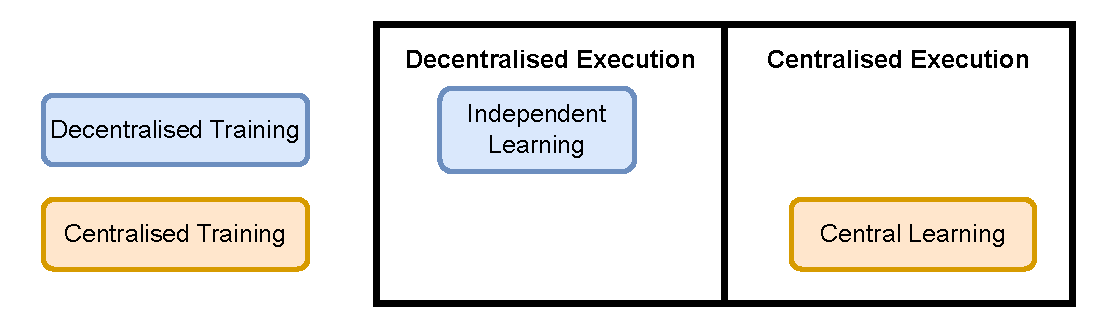
\includegraphics[width=\textwidth]{images/marl_paradigms_no_ctde.pdf}}
%         \only<2->{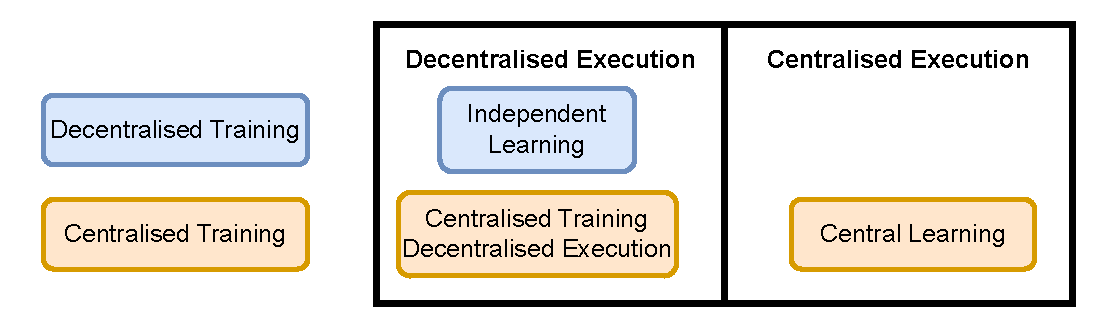
\includegraphics[width=\textwidth]{images/marl_paradigms.pdf}}
%     \end{figure}
%
%     \vspace{-1em}
%
%     \visible<2->{
%     }
%
%     % \visible<3->{
%     %     What about decentralised training and centralised execution? Impractical since execution is typically more constrained than training.
%     % }
%
%     \visible<3->{
%         For multi-agent deep RL algorithms, we will focus on algorithms under decentralised execution.
%     }
% \end{frame}

\section{Independent Learning with Deep Reinforcement Learning}

\begin{frame}[t]{Independent Learning with Deep Reinforcement Learning}
    \begin{reminderbox}
        In the independent learning framework, each agent $i$ learns its policy $\pi_i$ using only its local history of observations, treating the effects of other agents' actions as part of the environment.

        \blist
            \item From the perspective of the individual agent, the environment transition function looks like this:
        \elist
        \vspace{5pt}
        \[
        \mathcal{T}_i(s^{t+1} | s^t, a_i) \propto \sum_{a_{-i} \in A_{-i}} \mathcal{T}(s^{t+1} | s^t, \langle a_i, a_{-i} \rangle) \prod_{j \neq i} \pi_j(a_j | s^t)
        \]
    \end{reminderbox}

    % \vspace{2em}

    \visible<2->{
        How about we do this with deep RL? We have already seen several single-agent deep RL algorithms: \only<2>{DQN}\only<3>{\e{DQN}}, REINFORCE, \only<2>{A2C}\only<3>{\e{A2C}}, PPO, etc.
    }

\end{frame}

\begin{frame}[t]{Independent Deep Q-Networks}
    \scalebox{0.60}{
        \begin{minipage}{0.95\linewidth}
            \balg{Independent deep Q-networks}{IDQN}
                    \State Initialize $n$ value networks with random parameters $\theta_1,\dots,\theta_n$
                    \State Initialize $n$ target networks with parameters $\widebar\theta_1=\theta_1,\dots,\widebar\theta_n=\theta_n$
                    \State Initialize a replay buffer for each agent $D_1, D_2, \dots, D_n$
                    \For{time step $t=0, 1, 2, \dots$}
                        \State Collect current observations $\ob^t_1, \dots, \ob^t_n$
                        \For{agent $i=1, \dots, n$}
                            \State With probability $\epsilon$: choose random action $\ac^t_i$
                            \State Otherwise: choose $\ac^t_i \in \argmax_{\ac_i}{Q(\his^t_i, \ac_i; \theta_i)}$
                        \EndFor
                        \State Apply actions $(\ac^t_1,\ldots,\ac^t_n)$; collect rewards $\rew^t_1,\ldots,\rew^t_n$ and next observations $\ob^{t+1}_1,\ldots,\ob^{t+1}_n$
                        \For{agent $i=1,\dots, n$}
                            \State Store transition $(\his^t_i, \ac^t_i, \rew^t_i, \his^{t+1}_i)$ in replay buffers $D_i$
                            \State Sample random mini-batch of $\batchsize$ transitions $(\his^{k}_i, \ac^{k}_i, \rew^{k}_i, \his^{k+1}_i)$ from $D_i$
                            \If{$\st^{k+1}$ is terminal}
                                \State Targets $y^k_i \gets \rew^k_i$
                            \Else
                                \State Targets $y^k_i \gets \rew^k_i + \dsc \max_{\ac'_i\in\Ac_i} Q(\his^{k+1}_i, \ac'_i; \widebar{\theta_i})$
                            \EndIf
                            \State Loss $\loss(\theta_i) \gets \frac{1}{\batchsize} \sum_{k=1}^\batchsize \biggl(y^k_i - Q(\his^k_i, \ac^k_i; \theta_i)\biggr)^2$
                            \State Update parameters $\theta_i$ by minimizing the loss $\loss(\theta_i)$
                            \State In a set interval, update target network parameters $\widebar\theta_i$
                        \EndFor
                    \EndFor
            \ealg
        \end{minipage}
    }
    \hfill
    \begin{minipage}{0.38\textwidth}
        \blist
            \item<2-> Almost identical to DQN from Chapter 8 but with $n$ agents!
            \item<3-> Replay buffer contains off-policy experiences due to changing policies
            \item<3-> In MARL, the policies of \e{all} agents are changing $\rightarrow$ training can be unstable
        \elist
    \end{minipage}
\end{frame}

\begin{frame}[t]{Independent Advantage Actor-Critic}
    \scalebox{0.55}{
        \begin{minipage}{0.95\linewidth}
            \vspace{-1em}
            \balg{Independent A2C with synchronous environments}{IA2C}
                    \State Initialize $n$ actor networks with random parameters $\phi_1,\dots,\phi_n$
                    \State Initialize $n$ critic networks with random parameters $\theta_1,\dots,\theta_n$
                    \State Initialize $K$ parallel environments 
                    \For{time step $t=0\dots$}
                        \State Batch of observations for each agent and environment: $\left[\begin{smallmatrix}\ob^{t,1}_1 \dots \ob^{t,K}_1 \\ \ddots\\ \ob^{t,1}_n \dots \ob^{t,K}_n   \end{smallmatrix}\right]$
                        \State Sample actions $\left[\begin{smallmatrix}\ac^{t,1}_1 \dots \ac^{t,K}_1 \\ \ddots\\ \ac^{t,1}_n \dots \ac^{t,K}_n\end{smallmatrix}\right] \sim \pol(\cdot \mid \his_1^{t};\phi_1), \ldots, \pol(\cdot \mid \his_n^{t};\phi_n)$
                        \State Apply actions; collect rewards $\left[\begin{smallmatrix}\rew^{t,1}_1 \dots \rew^{t,K}_1 \\ \ddots\\ \rew^{t,1}_n \dots \rew^{t,K}_n   \end{smallmatrix}\right]$ and observations $\left[\begin{smallmatrix}\ob^{t+1,1}_1 \dots \ob^{t+1,K}_1 \\ \ddots\\ \ob^{t+1,1}_n \dots \ob^{t+1,K}_n   \end{smallmatrix}\right]$
                        \For{agent $i=1,\dots, n$}
                            \If{$\st^{t+1,k}$ is terminal}
                                \State Advantage $Adv(\his^{t,k}_i, \ac^{t,k}_i) \gets \rew^{t,k}_i - V(\his^{t,k}_i; \theta_i)$
                                \State Critic target $y^{t,k}_i \gets \rew^{t,k}_i$
                            \Else
                                \State Advantage $Adv(\his^{t,k}_i, \ac^{t,k}_i) \gets \rew^{t,k}_i + \dsc V(\his^{t+1,k}_i; \theta_i) - V(\his^{t,k}_i; \theta_i)$
                                \State Critic target $y^{t,k}_i \gets \rew^{t,k}_i + \dsc V(\his^{t+1,k}_i; \theta_i)$
                            \EndIf
                            \State Actor loss $\loss(\phi_i) \gets \frac{1}{K} \sum_{k=1}^K Adv(\his^{t,k}_i, \ac^{t,k}_i) \log \pol(\ac^{t,k}_i \mid \his^{t,k}_i; \phi_i)$
                            \State Critic loss $\loss(\theta_i) \gets \frac{1}{K} \sum_{k=1}^K \left(y^{t,k}_i - V(\his^{t,k}_i; \theta_i)\right)^2$
                            \State Update parameters $\phi_i$ by minimizing the actor loss $\loss(\phi_i)$
                            \State Update parameters $\theta_i$ by minimizing the critic loss $\loss(\theta_i)$
                        \EndFor
                    \EndFor
            \ealg
        \end{minipage}
    }
    \hfill
    \begin{minipage}{0.38\textwidth}
        \blist
            \item<2-> Almost identical to single-agent A2C from Chapter 8
            \item<3-> Similar adaptation can be done for independent REINFORCE and independent PPO
        \elist
    \end{minipage}
\end{frame}

\begin{frame}[t]{Challenges of Multi-Agent Reinforcement Learning}
    \begin{reminderbox}
        MARL algorithms suffer from multi-agent specific challenges:
        \blist
            \item \fat{Non-stationarity}: exacerbated due to changing policies of all agents
            \item \fat{Equilibrium selection}: how to converge to a stable equilibrium?
            \item \fat{Multi-agent credit assignment}: how to attribute rewards to agents' actions? (especially in common-reward settings)
            \item \fat{Scaling to many agents}: how to efficiently scale to large numbers of agents?
        \elist
    \end{reminderbox}

    \visible<2->{
        Centralised training with decentralised execution (CTDE) can help address some of these challenges.
    }
\end{frame}

\section{Multi-Agent Policy Gradient Algorithms}

\begin{frame}[t]{The Policy-Gradient Theorem}
    \begin{reminderbox}
        Follow this gradient to optimise the parameters $\phi$ of the policy $\pol$ to maximise the expected return:
        \begin{align*}
            \gradient_\phi J(\phi) &\propto \sum_{\st\in\St} \pr(\st \mid \pol) \sum_{\ac\in\Ac} Q^\pol(\st, \ac) \gradient_\phi \pol(\ac \mid \st; \phi)\\
                                   &= \ex{\st \sim \pr(\cdot \mid \pol), \ac \sim \pol(\cdot \mid \st; \phi)}{Q^\pol(\st, \ac) \gradient_\phi \log \pol(\ac \mid \st; \phi)}
        \end{align*}
    \end{reminderbox}

    \vspace{1em}

    \visible<2->{
        Does this also hold for MARL?
        \visible<3->{
            Yes, with minor modifications!
        }
    }
\end{frame}

\begin{frame}[t]{The Multi-Agent Policy-Gradient Theorem}
    \begin{solutionbox}
        In MARL, the expected returns of agent $i$ under its policy $\pol_i$ depends on the policies of all other agents $\pol_{-i}$ $\rightarrow$ the multi-agent policy gradient theorem defines an expectation over the policies of \fat{all} agents:
        \visible<2->{
            \begin{equation*}
                \gradient_{\phi_i} J(\phi_i) \propto \ex{\fhis\sim \cpr{\fhis}{\pol}, \ac_i \sim \pol_i, \jac_{-i} \sim \pol_{-i}}{Q_i^\pol(\fhis, \con{\ac_i, \jac_{-i}}) \gradient_{\phi_i} \log \pol_i(\ac_i \mid \his_i = \obsext_i(\fhis); \phi_i)}
            \end{equation*}
        }
        \vspace{-1.5em}
    \end{solutionbox}

    \visible<3->{
        $\rightarrow$ Derive policy update rules by finding estimators for expected returns $Q_i^\pol(\fhis, \con{\ac_i, \jac_{-i}})$.
    }

    \visible<4->{
        We have already seen independent A2C that estimates $Adv(\his_i, \ac_i) \propto Q_i^\pol(\fhis, \con{\ac_i, \jac_{-i}})$.
    }

    \visible<5->{
        But can we do better? Perhaps by leveraging more information?
    }

\end{frame}

\begin{frame}[t]{Centralized Critics}
    \begin{notebox}
        In actor-critic algorithms, only the policy/actor is used during execution and the critic is used only during training $\rightarrow$ the critic can be conditioned on centralised information $\ci$ without compromising decentralised execution.
    \end{notebox}

    \visible<2->{
        This might include:
        \blist
            \item Global state $\st$
            \item Joint action $\jac$
            \item Joint observation history $\his$
            \item \dots
        \elist
    }
\end{frame}

\begin{frame}[t]{Centralized Critics}
    \begin{figure}[t]
        \centering
        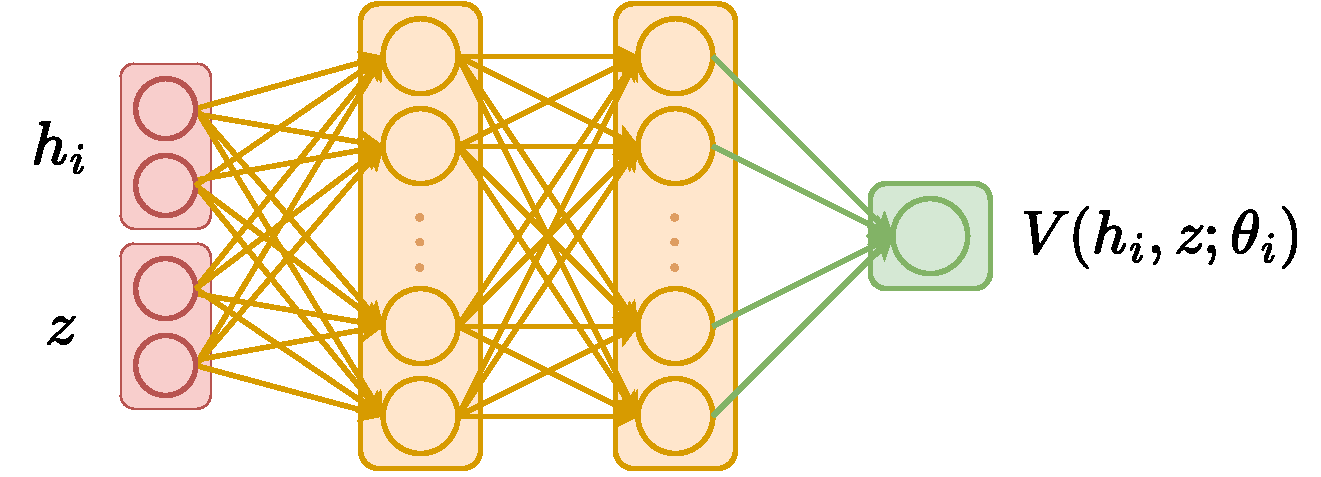
\includegraphics[width=.8\linewidth]{images/chapter_9/v_architecture.pdf}
    \end{figure}

    \visible<2->{
        Now we can integrate centralized critics into multi-agent policy gradient algorithms.
    }
\end{frame}

\begin{frame}[t]{Centralized Advantage Actor-Critic}
    \scalebox{0.50}{
        \begin{minipage}{0.95\linewidth}
            \balg{Centralized A2C with synchronous environments}{centralv}
                \State Initialize $n$ actor networks with random parameters $\phi_1,\dots,\phi_n$
                \State Initialize $n$ critic networks with random parameters $\theta_1,\dots,\theta_n$
                \State Initialize $K$ parallel environments 
                \For{time step $t=0\dots$}
                    \State Batch of observations for each agent and environment: $\left[\begin{smallmatrix}\ob^{t,1}_1 \dots \ob^{t,K}_1 \\ \ddots\\ \ob^{t,1}_n \dots \ob^{t,K}_n   \end{smallmatrix}\right]$
                    \State {\color{red} Batch of centralized information for each environment: $\left[\ci^{t,1} \dots \ci^{t,K}\right]$}
                    \State Sample actions $\left[\begin{smallmatrix}\ac^{t,1}_1 \dots \ac^{t,K}_1 \\ \ddots\\ \ac^{t,1}_n \dots \ac^{t,K}_n\end{smallmatrix}\right] \sim \pol(\cdot \mid \his_1^{t};\phi_1), \ldots, \pol(\cdot \mid \his_n^{t};\phi_n)$
                    \State Apply actions; collect rewards $\left[\begin{smallmatrix}\rew^{t,1}_1 \dots \rew^{t,K}_1 \\ \ddots\\ \rew^{t,1}_n \dots \rew^{t,K}_n   \end{smallmatrix}\right]$, observations $\left[\begin{smallmatrix}\ob^{t+1,1}_1 \dots \ob^{t+1,K}_1 \\ \ddots\\ \ob^{t+1,1}_n \dots \ob^{t+1,K}_n   \end{smallmatrix}\right]$, {\color{red} and centralized information $\left[\ci^{t+1,1} \dots \ci^{t+1,K}\right]$}
                    \For{agent $i=1,\dots, n$}
                        \If{$\st^{t+1,k}$ is terminal}
                            \State $Adv(\his^{t,k}_i, {\color{red} \ci^{t,k}}, \ac^{t,k}_i) \gets \rew^{t,k}_i - V(\his^{t,k}_i, {\color{red}\ci^{t,k}}; \theta_i)$
                            \State Critic target $y^{t,k}_i \gets \rew^{t,k}_i$
                        \Else
                            \State $Adv(\his^{t,k}_i, {\color{red} \ci^{t,k}}, \ac^{t,k}_i) \gets \rew^{t,k}_i + \dsc V(\his^{t+1,k}_i, {\color{red} \ci^{t+1,k}}; \theta_i) - V(\his^{t,k}_i, {\color{red} \ci^{t,k}}; \theta_i)$
                            \State Critic target $y^{t,k}_i \gets \rew^{t,k}_i + \dsc V(\his^{t+1,k}_i, {\color{red} \ci^{t+1,k}}; \theta_i)$
                        \EndIf
                        \State Actor loss $\loss(\phi_i) \gets \frac{1}{K} \sum_{k=1}^K Adv(\his^{t,k}_i, {\color{red} \ci^{t,k}}, \ac^{t,k}_i) \log \pol(\ac^{t,k}_i \mid \his^{t,k}_i; \phi_i)$
                        \State Critic loss $\loss(\theta_i) \gets \frac{1}{K} \sum_{k=1}^K \left(y^{t,k}_i - V(\his^{t,k}_i, {\color{red} \ci^{t,k}}; \theta_i)\right)^2$
                        \State Update parameters $\phi_i$ by minimizing the actor loss $\loss(\phi_i)$
                        \State Update parameters $\theta_i$ by minimizing the critic loss $\loss(\theta_i)$
                    \EndFor
                \EndFor
            \ealg
        \end{minipage}
    }
    \hfill
    \begin{minipage}{0.38\textwidth}
        \blist
            \item Simple extension of independent A2C.
            \item Centralized information $\ci$ is added to the critic input.
        \elist
    \end{minipage}
\end{frame}

\begin{frame}[t]{Centralized Critics in Action}

    \begin{figure}
        \centering
        \begin{subfigure}[b]{0.34\textwidth}
            \centering
            \raisebox{15pt}{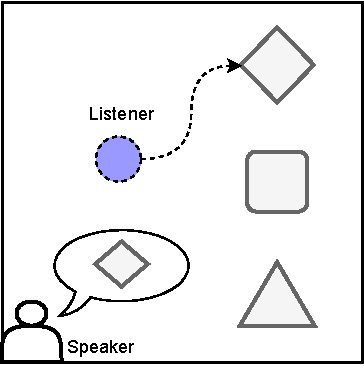
\includegraphics[width=0.8\textwidth]{images/chapter_9/speaker-listener.pdf}}
            \caption{Speaker-listener game}
        \end{subfigure}
        \hfill
        \begin{subfigure}[b]{0.65\textwidth}
            \centering
            \visible<2->{
                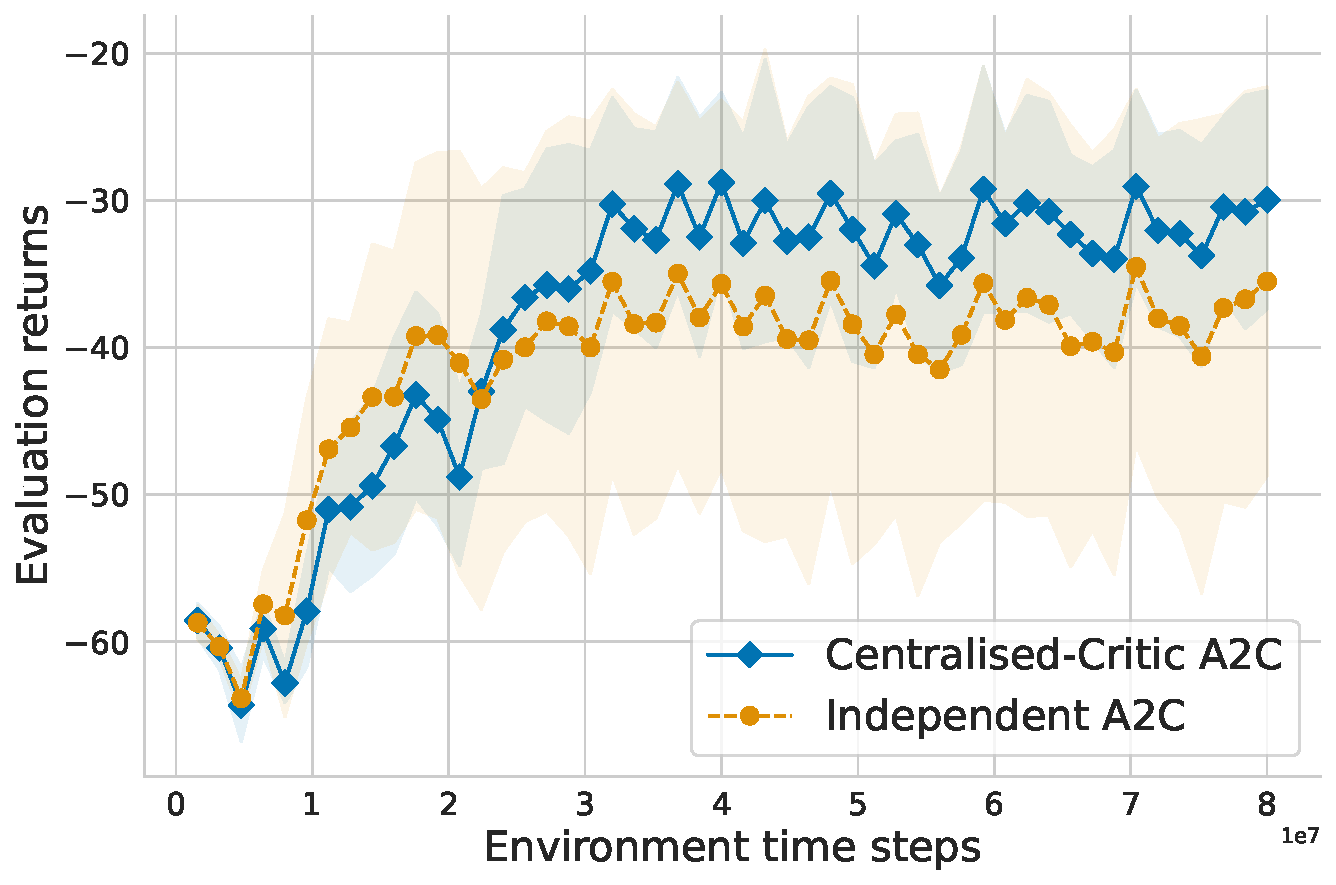
\includegraphics[width=0.8\textwidth]{images/chapter_9/centralv-speaker-listener.pdf}
                \caption{Training curves}
            }
        \end{subfigure}
        \vspace{-1.5em}
    \end{figure}

    \vspace{-.5em}
    \visible<2->{
        Agents with centralized critics converge to higher returns than agents with independent critics in the partially observable speaker-listener game.
    }
\end{frame}

\begin{frame}[t]{Centralized Action-Value Critics}
    Similarly, we can learn an action-value function that receives additional centralized information $\ci$.

    \begin{figure}[t]
        \centering
        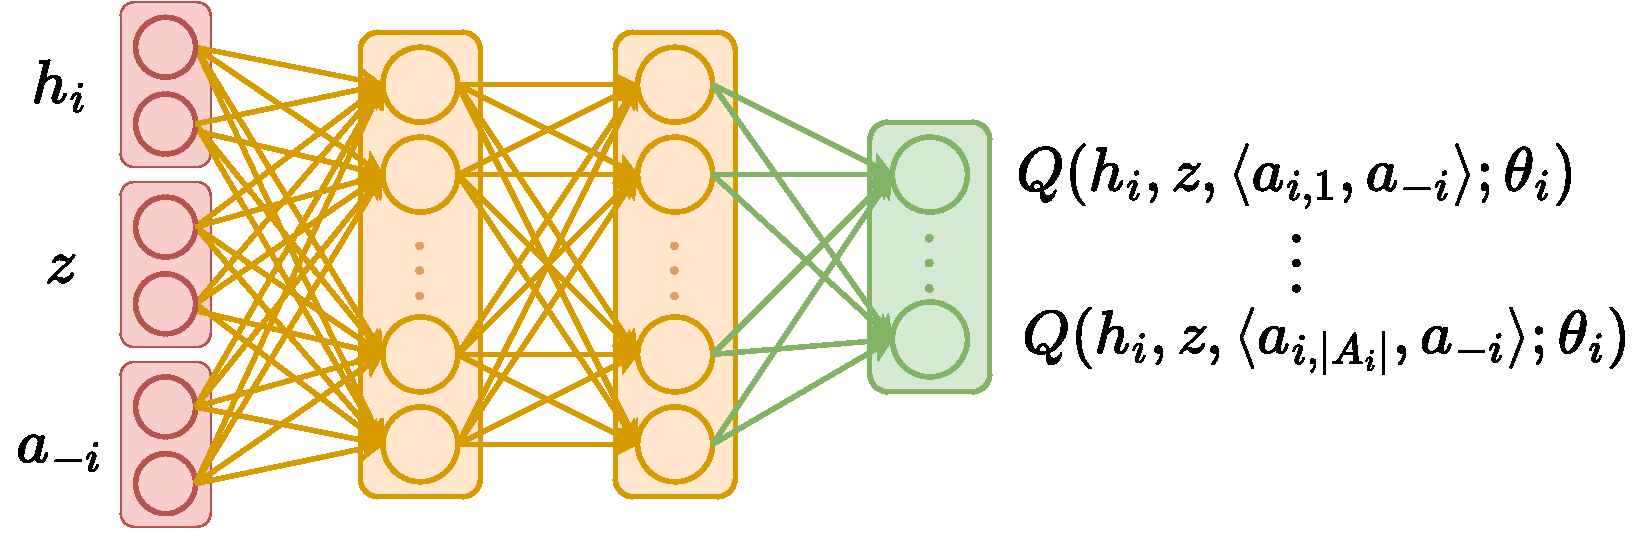
\includegraphics[width=.8\linewidth]{images/chapter_9/macac_architecture.pdf}
    \end{figure}

    \visible<2->{
        But what for? The centralized action-value critic can reason about the joint action space!
    }
\end{frame}

\begin{frame}[t]{Counterfactual Multi-Agent Policy Gradient}
    For example, we can compute a counterfactual advantage for agent $i$
    \begin{equation*}
        Adv_i(\his_i, \ci, \jac) = Q(\his_i, \ci, \jac; \theta) - \underbrace{\sum_{\ac^\prime_i \in \Ac_i} \pol(\ac^\prime_i \mid \his_i; \phi_i) Q(\his_i, \ci, \con{\ac^\prime_i, \ac_{-i}}; \theta)}_{\text{counterfactual baseline}}
    \end{equation*}

    \vspace{-1em}
    with the following components:

    \blist
        \item<2-> $Q(\his_i, \ci, \jac; \theta)$: expected returns when applying joint action $\jac$ $\rightarrow$ agent $i$ applies action $\ac_i$ and all other agents apply actions $\ac_{-i}$
        \item<3-> Counterfactual baseline: expected returns when agent $i$ samples its action $\ac^\prime_i$ from its policy $\pol(\cdot; \phi_i)$ and all other agents apply their actual actions $\ac_{-i}$
    \elist

    \visible<4->{
        This allows us to identify the contribution of agent $i$'s action $\ac_i$ to received rewards and, thus, can help to address the \e{credit assignment problem} in common-reward games.
    }
\end{frame}

\begin{frame}[t]{The Equilibrium Selection Problem}
    \begin{problembox}
        Many multi-agent games have multiple equilibria. In such games, it difficult for all agents to agree on and stably converge to a single equilibrium. This is known as the \e{equilibrium selection problem}.
    \end{problembox}

    \vspace{1em}

    \visible<2->{
        \begin{minipage}{.25\textwidth}
            \begin{figure}[h]
                \centering
                \gametwo{A & B}{A & 4,4\ddag & 0,3}{B & 3,0 & 2,2\dag}
                \caption{Stag Hunt}
            \end{figure}
        \end{minipage}
        \begin{minipage}{.3\textwidth}
            \begin{figure}[h]
                \centering
                \gamethree{A & B & C}{A & 11\ddag & -30 & 0}{B & -30 & 7\dag & 0}{C & 0 & 6 & 5}
                \caption{Climbing}
            \end{figure}
        \end{minipage}
        \begin{minipage}{.4\textwidth}
            The Stag Hunt and Climbing matrix games have multiple equilibria.\\
            \dag: Pareto-dominated equilibria\\
            \ddag: Pareto-optimal equilibria
        \end{minipage}
    }
\end{frame}

\begin{frame}[t]{Example for the Equilibrium Selection Problem}
    \begin{columns}
        \begin{column}{.40\textwidth}
            \begin{figure}
                \centering
                \gamethree{A & B & C}{A & 11\ddag & -30 & 0}{B & -30 & 7\dag & 0}{C & 0 & 6 & 5}
                \caption{Climbing game}
            \end{figure}

            \vspace{1em}
            \blist
                \item Pareto-optimal equilibrium (\ddag): (A, A) with +11
                \item Pareto-dominated equilibrium (\dag): (B, B) with +7
            \elist
        \end{column}
        \begin{column}{.60\textwidth}
            \blist
                \item<2-> All agents prefer the Pareto-optimal equilibrium
                    \item<2-> \fat{But} deviation from the equilibrium by any agent results in lower returns $\rightarrow$ e.g. risk of receiving -30 if one agent deviates from action A to action B
            \elist

            \vspace{-.5em}

            \visible<3->{
                \begin{problembox}
                    Due to the risk of deviations, agents often converge to the safer Pareto-dominated equilibrium or even the suboptimal solution (C, C) with +5.
                \end{problembox}
            }

            \visible<4->{
                How can we overcome this problem and robustly converge to the optimal equilibrium?
            }
        \end{column}
    \end{columns}
\end{frame}

\begin{frame}[t]{Pareto Actor-Critic for Equilibrium Selection}
    Both shown matrix games are \e{no-conflict games} where agents agree on the optimal policy:
    \begin{equation*}
        \argmax_\pi \exret_i(\pi) = \argmax_\pi \exret_j(\pi) \quad \forall i,j \in \Ag
    \end{equation*}

    \visible<2->{
        We can use this property! Agent $i$ during training assumes that all other agents follow the policy $\pol^+_{-i}$ that is best for agent $i$, i.e.\ $\pi^+_{-i} \in \argmax_{\pi_{-i}} \exret_i(\pi_i, \pi_{-i})$.
    }

    \visible<3->{
        We can compute $\pi^+_{-i}$ using a centralized critic that receives the joint action $\jac$ as input:
        \vspace{-.5em}
        \begin{equation*}
            \pi_{-i}^+ \in \argmax_{\jac_{-i}}Q(\his^{t}_i, \ci^t, \con{\ac^t_{i}, \jac_{-i}})
        \end{equation*}
        \vspace{-.5em}
    }
    \visible<4->{
        During training, agent $i$ optimises its policy $\pol_i$ by minimising the following loss:
        \begin{equation*}
            \mathcal{L}(\phi_i) 
            = -\ex{\ac^t_i\sim\pol_i, \ac^t_{-i}\sim\pol^+_{-i}}{\log\pol(\ac^t_i \mid \his_i^{t}; \phi_i) \left(Q^{\pi^+}(\his^{t}_i, \ci^t, \con{a_i^t, a_{-i}^t}; \theta_i^q)  -V^{\pi^+}(\his^{t}_i, \ci^t; \theta_i^v)\right)}
        \end{equation*}
    }
\end{frame}

\begin{frame}[t]{Pareto Actor-Critic for Equilibrium Selection in Climbing Game}
    \vspace{1em}

    \begin{minipage}{.6\textwidth}
        \begin{figure}
            \centering
            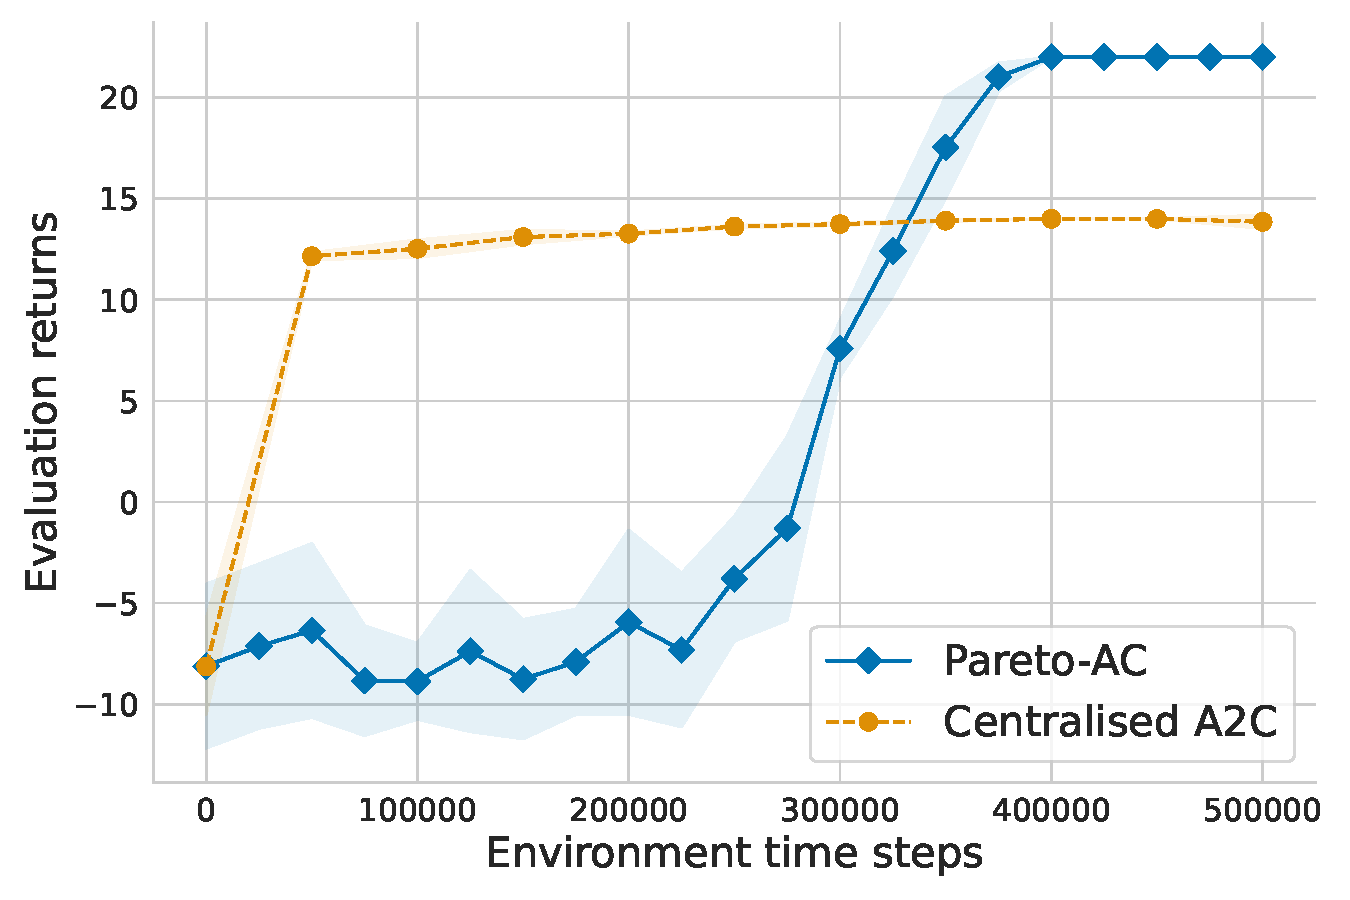
\includegraphics[width=0.8\textwidth]{images/chapter_9/pac-climbing.pdf}
            \caption{Learning curves in the Climbing game.}
        \end{figure}
    \end{minipage}
    \begin{minipage}{.39\textwidth}
        \blist
            \item<2-> A2C with centralized state-value critic converges to the Pareto-dominated equilibrium (B, B) with +7 (per agent).
            \item<3-> \e{Pareto actor-critic} converges to the Pareto-optimal equilibrium (A, A) with +11 (per agent).
        \elist
    \end{minipage}
\end{frame}

\section{Value Decomposition in Common-Reward Games}

\begin{frame}[t]{Centralized Value Functions in Value-Based MARL}
    We addressed MARL challenges in policy gradient algorithms by leveraging centralized critics. Can we also use centralized value functions in value-based MARL algorithms?

    \visible<2->{
        \begin{problembox}
            In value-based MARL algorithms, e.g.\ IDQN, agents learn value functions and derive their policy from them. However, learning and deriving a policy from centralized value functions would prevent decentralized execution.
        \end{problembox}
    }

    \visible<3->{
        How can we overcome this limitation and leverage the benefits of centralized value functions in value-based MARL algorithms?
    }
\end{frame}

\begin{frame}[t]{Value Decomposition}
    We will focus on \e{value decomposition} methods for common-reward games. These methods aim to decompose a centralized action-value function of all agents
    \begin{equation*}
        Q(\his^t, \ci^t, \jac^t; \theta) = \ex{}{\sum_{\tau=t}^\infty \dsc^{\tau-t} \rew^\tau \mid \his^t, \ci^t, \jac^t}
    \end{equation*}
    into individual utility functions of each agent: $Q(\his_i, \ac_i; \theta_i)$ for $i\in\Ag$

    \visible<2->{
        This decomposition has several benefits:
        \blist
            \item Agents benefit from centralized information during training
            \item Simplify learning by decomposing the centralized value function
            \item Agents learn their individual utility functions to represent their contribution to the centralized value function, helping to address the \fat{credit assignment problem}
        \elist
    }
\end{frame}

\begin{frame}[t]{Individual-Global-Max Property}
    How do we ensure that decentralized action selection with respect to the agents' individual utility functions leads to effective joint actions with respect to the decomposed centralized action-value function?

    \visible<2->{
        \begin{solutionbox}
            Let $\fhis$ be a full history with joint-observation histories $\his = \obsext(\fhis)$, individual observation histories, $\his_i = \obsext_i(\fhis)$, and centralized information $\ci$. The \e{individual-global-max (IGM) property} is satisfied if and only if:
            \begin{equation*}
                \forall \jac = (\ac_1, \ldots, \ac_n) \in \Ac: \jac \in \Ac^*(\his, \ci; \theta) \iff \forall i \in \Ag: \ac_i \in \Ac^*_i(\his_i; \theta_i)
            \end{equation*}
            with $\Ac^*(\his, \ci; \theta) = \argmax_{\jac \in \Ac} Q(\his, \ci, \jac; \theta)$ and $\Ac^*_i(\his_i; \theta_i) = \argmax_{\ac_i \in \Ac_i} Q(\his_i, \ac_i; \theta_i)$.
        \end{solutionbox}
    }
\end{frame}

\begin{frame}[t]{The Importance of the Individual-Global-Max Property}
    Upholding the IGM property has two important implications:
    \begin{enumerate}
        \item<2-> If all agents decentrally select actions that maximise their individual utility functions, the resulting joint action will maximise the centralized action-value function $\rightarrow$ \e{effective decentralised execution}
        \item<3-> The greedy joint action with respect to the centralized action-value function can be efficiently obtained by selecting the greedy action for each agent with respect to their individual utility functions $\rightarrow$ \e{efficient centralized training}
    \end{enumerate}

    \visible<4->{
        \begin{notebox}
            It is not guaranteed that for a given environment, there exists a decomposition of the centralized action-value function that satisfies the IGM property.
        \end{notebox}
    }
\end{frame}

\begin{frame}[t]{Linear Value Decomposition}
    \e{Value decomposition networks} (VDN) uses a simple linear decomposition of the centralized action-value function:
    \begin{equation*}
        Q(\his^t, \ci^t, \jac^t; \theta) = \sum_{i\in\Ag} Q(\his^t_i, \ac^t_i; \theta_i)
    \end{equation*}

    \visible<2->{
        This decomposition satisfies the IGM property and we can jointly optimise the parameters of all networks by minimising the following loss on sampled batches of experiences $\batch$:
        \begin{equation*}
            \loss(\theta) = \frac{1}{\batchsize} \sum_{(\his^t, \jac^t, \rew^t, \his^{t+1}) \in \batch} \left(\rew^t + \dsc \sum_{i\in\Ag}{\max_{\ac_i\in\Ac_i}{Q(\his_i^{t+1}, \ac_i; \bar\theta_i)}} - \sum_{i\in\Ag}{Q(\his_i^t, \ac_i^t; \theta_i)}\right)^2
        \end{equation*}
        with $\bar\theta_i$ denoting the parameters of agent $i$'s target network.
    }
\end{frame}

\begin{frame}[t]{Value Decomposition Networks}
    \scalebox{0.6}{
        \begin{minipage}{0.95\linewidth}
            \balg{Value decomposition networks (VDN)}{VDN}
                \State Initialize $n$ utility networks with random parameters $\theta_1,\dots,\theta_n$
                \State Initialize $n$ target networks with parameters $\widebar\theta_1=\theta_1,\dots,\widebar\theta_n=\theta_n$
                \State Initialize a shared replay buffer $D$
                \For{time step $t=0, 1, 2, \dots$}
                    \State Collect current observations $\ob^t_1,\dots, \ob^t_n$
                    \For{agent $i=1,\dots, n$}
                        \State With probability $\epsilon$: choose random action $\ac^t_i$
                        \State Otherwise: choose $\ac^t_i \in \argmax_{\ac_i}{Q(\his^t_i, \ac_i; \theta_i)}$
                    \EndFor
                    \State Apply actions; collect shared reward $\rew^t$ and next observations $\ob^{t+1}_1,\ldots,\ob^{t+1}_n$
                    \State Store transition $(\his^t, \jac^t, \rew^t, \his^{t+1})$ in shared replay buffer $D$
                    \State Sample mini-batch of $\batchsize$ transitions $(\his^{k}, \jac^{k}, \rew^{k}, \his^{k+1})$ from $D$
                    % \If{$\his^{k+1}$ is terminal}
                    \If{$\st^{k+1}$ is terminal}
                        \State Targets $y^k \gets \rew^k$
                    \Else
                        \State Targets $y^k \gets \rew^k + \dsc \sum_{i\in\Ag}\max_{\ac'_i\in\Ac_i} Q(\his^{k+1}_i, \ac'_i; \widebar{\theta_i})$
                    \EndIf
                    \State Loss $\loss(\theta) \gets \frac{1}{\batchsize} \sum_{k=1}^\batchsize \biggl(y^k - \sum_{i\in\Ag} Q(\his^k_i, \ac^k_i; \theta_i)\biggr)^2$
                    \State Update parameters $\theta$ by minimizing the loss $\loss(\theta)$
                    \State In a set interval, update target network parameters $\widebar\theta_i$ for each agent $i$
                \EndFor
            \ealg
        \end{minipage}
    }
    \hspace{1em}
    \begin{minipage}{0.3\textwidth}
        \begin{figure}
            \centering
            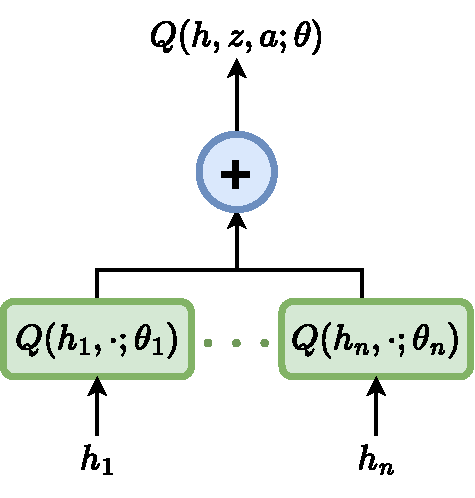
\includegraphics[width=\textwidth]{images/chapter_9/vdn_architecture.pdf}
        \end{figure}
    \end{minipage}
\end{frame}

\begin{frame}[t]{Monotonic Value Decomposition}
    A more general decomposition (that also ensures the IGM property) can be formulated by assuming that the centralized action-value function is a (strictly) monotonically increasing function with respect to any individual utility function:
    \begin{equation*}
        \forall i\in\Ag, \forall \jac \in \Ac: \frac{\partial Q(\his, \ci, \jac; \theta)}{\partial Q(\his_i, \ac_i; \theta_i)} > 0
    \end{equation*}

    \visible<2->{
        The \e{QMIX} algorithm implements this assumption using a mixing function $f_{\text{mix}}$ that aggregates individual utilities to approximate the centralized action-value function:
        \begin{equation*}
            Q(\his, \ci, \jac, \theta) = f_{\text{mix}}\left(Q(\his_1, \ac_1; \theta_1), \ldots, Q(\his_n, \ac_n; \theta_n); \theta_{\text{mix}}\right)
        \end{equation*}
    }
\end{frame}

\begin{frame}[t]{QMIX Architecture}
    \begin{figure}[h]
        \centering
        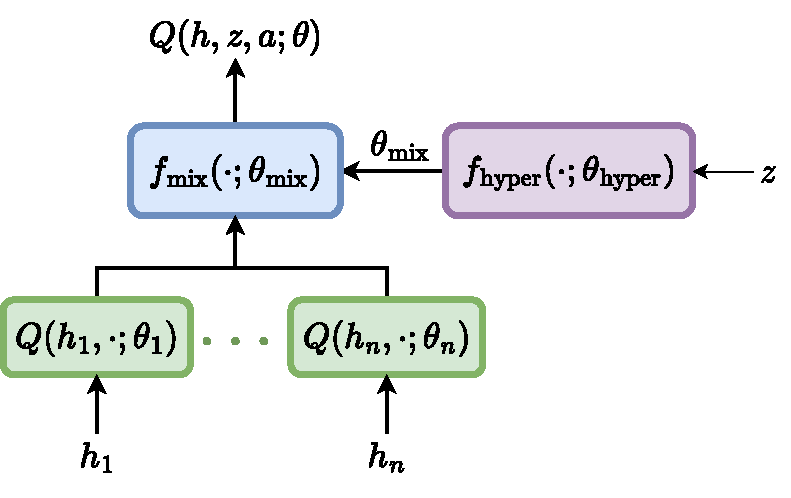
\includegraphics[width=.5\textwidth]{images/chapter_9/qmix_architecture.pdf}
    \end{figure}

    \vspace{-1em}

    The centralized action-value function is monotonic with respect to individual utilities if all weights of $f_{\text{mix}}$ are positive $\rightarrow$ ensure positive weights by obtaining the parameters of the mixing function from a hypernetwork $f_{\text{hyper}}$ conditioned on centralized information $\ci$

\end{frame}

\begin{frame}[t]{QMIX Optimisation}
    The parameters of all utility functions and the hypernetwork are jointly optimised by minimising the following loss on batches of experiences $\batch$ sampled from a replay buffer:
    \begin{equation*}
        \loss(\theta) = \frac{1}{\batchsize} \sum_{(\his^t, \ci^t, \jac^t, \rew^t, \his^{t+1}, \ci^{t+1}) \in \batch} \left(\rew^t + \dsc \max_{\jac\in\Ac}{Q(\his^{t+1}, \ci^{t+1}, \jac; \bar\theta)} - Q(\his^t, \ci^t, \jac^t; \theta)\right)^2
    \end{equation*}
    with the following decomposed value estimates:
    \begin{align*}
        Q(\his^t, \ci^t, \jac^t, \theta) &= f_{\text{mix}}\left(Q(\his^t_1, \ac^t_1; \theta_1), \ldots, Q(\his^t_n, \ac^t_n; \theta_n); \theta_{\text{mix}}\right)\\
        \max_{\jac\in\Ac}{Q(\his^{t+1}, \ci^{t+1}, \jac; \bar\theta)} &= f_{\text{mix}}\left(\max_{\ac_1\in\Ac_1} Q(\his^{t+1}_1, \ac_1; \bar\theta_1), \ldots, \max_{\ac_n\in\Ac_n} Q(\his^{t+1}_n, \ac_n; \bar\theta_n); \bar\theta_{\text{mix}}\right)
    \end{align*}
\end{frame}

% \begin{frame}[t]{QMIX -- Pseudocode}
%     \scalebox{0.48}{
%         \begin{minipage}{0.95\linewidth}
%             \balg{QMIX}{QMIX}
%                 \State Initialize $n$ utility networks with random parameters $\theta_1,\dots,\theta_n$
%                 \State Initialize $n$ target networks with parameters $\widebar\theta_1=\theta_1,\dots,\widebar\theta_n=\theta_n$
%                 \State Initialize hypernetwork with random parameters $\theta_\text{hyper}$
%                 \State Initialize a shared replay buffer $D$
%                 \For{time step $t=0, 1, 2, \dots$}
%                     \State Collect current centralized information $\ci^t$ and observations $\ob^t_1,\dots, \ob^t_n$
%                     \For{agent $i=1,\dots, n$}
%                         \State With probability $\epsilon$: choose random action $\ac^t_i$
%                         \State Otherwise: choose $\ac^t_i \in \argmax_{\ac_i}{Q(\his^t_i, \ac_i; \theta_i)}$
%                     \EndFor
%                     \State Apply actions; collect shared reward $\rew^t$, next centralized information $\ci^{t+1}$ and observations $\ob^{t+1}_1,\ldots,\ob^{t+1}_n$
%                     \State Store transition $(\his^t, \ci^t, \jac^t, \rew^t, \his^{t+1}, \ci^{t+1})$ in shared replay buffer $D$
%                     \State Sample mini-batch of $\batchsize$ transitions $(\his^k, \ci^k, \jac^{k}, \rew^{k}, \his^{k+1}, \ci^{k+1})$ from $D$
%                     % \If{$\his^{k+1}$ is terminal}
%                     \If{$\st^{k+1}$ is terminal}
%                         \State Targets $y^k \gets \rew^k$
%                     \Else
%                         \State Mixing parameters $\theta_\text{mix}^{k+1} \gets f_\text{hyper}(\ci^{k+1}; \theta_\text{hyper})$
%                         \State Targets $y^k \gets \rew^k + \dsc f_{\text{mix}}\left(
%                             \begin{array}{ll}
%                                 \max_{\ac'_1} Q(\his_1^{k+1}, \ac'_1; \widebar{\theta}_1),\\
%                                 \ddots\\
%                                 \max_{\ac'_n} Q(\his^{k+1}_n, \ac'_n; \widebar{\theta}_n)
%                             \end{array}
%                         ; \theta_{\text{mix}}^{k+1}\right)$
%                     \EndIf
%                     \State Mixing parameters $\theta_\text{mix}^k \gets f_\text{hyper}(\ci^k; \theta_\text{hyper})$
%                     \State Value estimates $Q(\his^k, \ci^k, \jac^k; \theta) \gets f_{\text{mix}}\left(Q(\his_1^k, \ac^k_1; \theta_1), \ldots, Q(\his_n^k, \ac^k_n; \theta_n); \theta_{\text{mix}}^k\right)$
%                     \State Loss $\loss(\theta) \gets \frac{1}{\batchsize} \sum_{k=1}^\batchsize \biggl(y^k - Q(\his^k, \ci^k, \jac^k; \theta)\biggr)^2$
%                     \State Update parameters $\theta$ by minimizing the loss $\loss(\theta)$
%                     \State In a set interval, update target network parameters $\widebar\theta_i$ for each agent $i$
%                 \EndFor
%             \ealg
%         \end{minipage}
%     }
% \end{frame}

\begin{frame}[t]{Value Decomposition in Matrix Games}
    To better understand how value decomposition works in practise, we will look at several exemplary tasks and the learned decompositions of both VDN and QMIX.

    \visible<2->{
        \begin{minipage}{0.25\textwidth}
            \begin{figure}
                \centering
                \gametwo{A & B}{A & 1 & 5}{B & 5 & 9}
                \caption{Linear game}
            \end{figure}
        \end{minipage}
        \hfill
        \begin{minipage}{0.29\textwidth}
            \begin{figure}
                \centering
                \gametwo{A & B}{A & 0 & 0}{B & 0 & 10}
                \caption{Monotonic game}
            \end{figure}
        \end{minipage}
        \hfill
        \begin{minipage}{0.4\textwidth}
            \begin{figure}
                \centering
                \gamethree{A & B & C}{A & 11 & -30 & 0}{B & -30 & 7 & 0}{C & 0 & 6 & 5}
                \caption{Climbing game}
            \end{figure}
        \end{minipage}
    }

    \visible<3->{
        \begin{table}
            \centering
            \small
            \begin{tabular}{l c c c}
                \toprule
                & \textbf{Linear game} & \textbf{Monotonic game} & \textbf{Climbing game} \\
                \midrule
                Linearly decomposable & \cmark & \xmark & \xmark \\
                Monotonically decomposable & \cmark & \cmark & \xmark \\
                \bottomrule
            \end{tabular}
        \end{table}
    }
    
\end{frame}

\begin{frame}[t]{Value Decomposition in Linearly Decomposable Matrix Game}
    \begin{figure}
        \centering
        \begin{subfigure}{0.2\textwidth}
            \centering
            \gametwo{A & B}{A & 1 & 5}{B & 5 & 9}
            \caption{True rewards}
        \end{subfigure}
        \begin{subfigure}{.39\textwidth}
            \centering
            \begin{tabular}{c?c|c}
                & $0.12$ & $\mathbf{4.12}$ \\
                \bhline
                $0.88$ & $1.00$ & $5.00$ \\
                \hline
                $\mathbf{4.88}$ & $5.00$ & $\mathbf{9.00}$ \\
            \end{tabular}
            \caption{VDN decomposition}
        \end{subfigure}
        \begin{subfigure}{.39\textwidth}
            \centering
            \begin{tabular}{c?c|c}
                & $-0.21$ & $\mathbf{0.68}$ \\
                \bhline
                $0.19$ & $1.00$ & $5.00$ \\
                \hline
                $\mathbf{0.96}$ & $5.00$ & $\mathbf{9.00}$ \\
            \end{tabular}
            \caption{QMIX decomposition}
        \end{subfigure}
    \end{figure}

    \visible<2->{
        We can make several observations from the learned decompositions:
        \blist
            \item<3-> VDN and QMIX are able to learn the true centralized action-value function
            \item<4-> The learned decompositions are not unique and can vary between different runs
            \item<5-> Individual utility values, in particular for QMIX, can be difficult to interpret (besides larger values indicating higher return estimates)
        \elist
    }
\end{frame}

\begin{frame}[t]{Value Decomposition in Monotonically Decomposable Matrix Game}
    \begin{figure}[t]
        \centering
        \begin{subfigure}{0.20\textwidth}
            \centering
            \gametwo{A & B}{A & 0 & 0}{B & 0 & 10}
            \caption{True rewards}
        \end{subfigure}
        \begin{subfigure}{.39\textwidth}
            \centering
            \begin{tabular}{c?c|c}
                & $-1.45$ & $\mathbf{3.45}$ \\
                \bhline
                $-0.94$ & $-2.43$ & $2.51$ \\
                \hline
                $\mathbf{4.08}$ & $2.60$ & $\mathbf{7.53}$ \\
            \end{tabular}
            \caption{VDN decomposition}
        \end{subfigure}
        \begin{subfigure}{.39\textwidth}
            \centering
            \begin{tabular}{c?c|c}
                & $-4.91$ & $\mathbf{0.82}$ \\
                \bhline
                $-4.66$ & $0.00$ & $0.00$ \\
                \hline
                $\mathbf{1.81}$ & $0.00$ & $\mathbf{10.00}$ \\
            \end{tabular}
            \caption{QMIX decomposition}
        \end{subfigure}
    \end{figure}

    \visible<2->{
        \begin{minipage}{.4\textwidth}
            \begin{figure}[t]
                \centering
                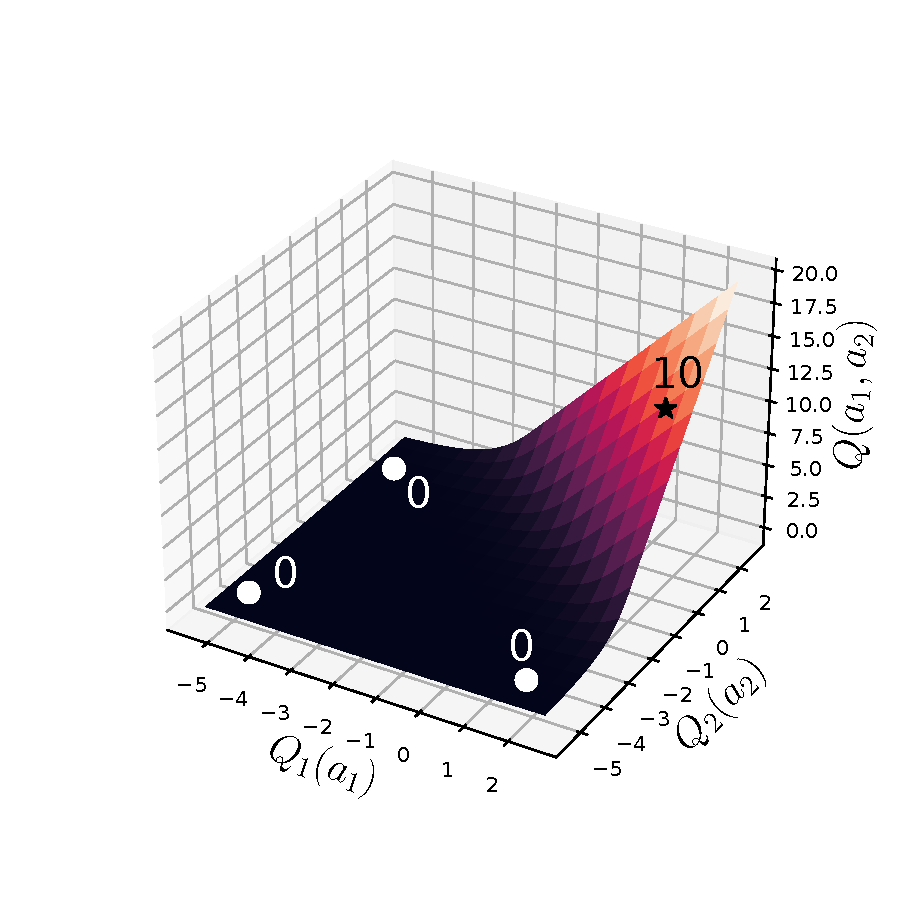
\includegraphics[width=.8\textwidth,trim=5em 5em 1em 5em,clip]{images/chapter_9/qmix_mixing3d.pdf}
            \end{figure}
        \end{minipage}
        \hfill
        \begin{minipage}{.57\textwidth}
            Only QMIX is able to represent the non-linear but monotonic relationship between the individual utility functions and the centralized action-value function.
        \end{minipage}
    }

\end{frame}

\begin{frame}[t]{Value Decomposition in Climbing Game}
    \begin{minipage}{.49\textwidth}
        \begin{figure}
            \centering
            \gamethree{A & B & C}{A & 11 & -30 & 0}{B & -30 & 7 & 0}{C & 0 & 6 & 5}
            \caption{True rewards}
        \end{figure}
    \end{minipage}
    \begin{minipage}{.49\textwidth}
        In the Climbing game, neither VDN nor QMIX are able to learn the true centralized action-value function and converge to sub-optimal policies.
    \end{minipage}

    \begin{figure}
        \begin{subfigure}{.49\textwidth}
            \centering
            \begin{tabular}{c?c|c|c}
                & $-4.56$ & $-4.15$ & $\mathbf{3.28}$ \\
                \bhline
                $-4.28$ & $-8.84$ & $-8.43$ & $-1.00$ \\
                \hline
                $-6.10$ & $-10.66$ & $-10.25$ & $-2.82$\\
                \hline
                $\mathbf{5.31}$ & $0.75$ & $1.16$ & $\mathbf{8.59}$\\
            \end{tabular}
            \caption{VDN decomposition}
        \end{subfigure}
        \begin{subfigure}{.49\textwidth}
            \centering
            \begin{tabular}{c?c|c|c}
                & $-16.60$ & $\mathbf{-0.24}$ & $-4.68$ \\
                \bhline
                $-7.44$ & $-11.16$ & $-11.16$ & $-11.16$ \\
                \hline
                $7.65$ & $-11.15$ & $2.34$ & $-1.37$\\
                \hline
                $\mathbf{11.27}$ & $-4.95$ & $\mathbf{8.72}$ & $5.01$\\
            \end{tabular}
            \caption{QMIX decomposition}
        \end{subfigure}
    \end{figure}
\end{frame}

\begin{frame}[t]{Value Decomposition in LBF}
    % (a) Visualization of the \lbf environment with two agents collecting three items in a $8\times8$ grid-world. The levels and starting locations of agents and items are randomized for each episode lasting up to twenty-five steps, and agents are rewarded with a shared reward for collecting up items. (b) Learning curves for IDQN, VDN, and QMIX in the \lbf environment. All algorithms are trained for two million environment steps using a learning rate of $\alpha = 3\cdot10^{-4}$, a batch size of 128, and a discount factor of $\dsc = 0.99$. The DQN value functions and individual utilities of VDN and QMIX are represented by a two-layer feedforward neural network with sixty-four hidden units and the ReLU activation function. The mixing network of QMIX is a two-layer feedforward neural network with thirty-two hidden units. All networks are shared between both agents \seehere{sec:parameter-sharing}. Target networks are updated every two hundred steps and the replay buffer contains the last \num{100000} transitions. All agents explore with an $\epsilon$-greedy policy with $\epsilon$ linearly annealed from $1$ to $0.05$ over training and a fixed $\epsilon=0.05$ being used during evaluation. Visualized learning curves and shading correspond to the mean and standard deviation across evaluation returns across five runs with different random seeds.

    So far, we looked at simple single-step matrix games. We will now compare IDQN, VDN and QMIX in a common-reward level-based foraging task where two agents need to collect three items in a $8\times8$ grid world:

    \begin{figure}
        \centering
        \begin{subfigure}{.39\textwidth}
            \centering
            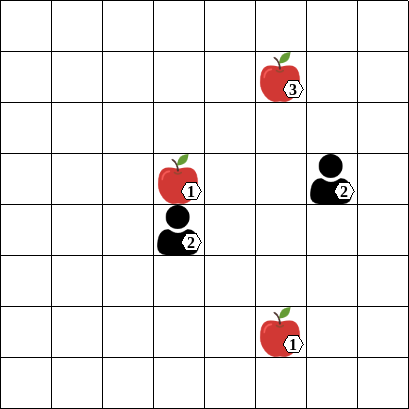
\includegraphics[width=.8\textwidth]{images/environments/lbf/lbf-8x8-2p-3f.png}
        \end{subfigure}
        \visible<2->{
            \begin{subfigure}{.59\textwidth}
                \centering
                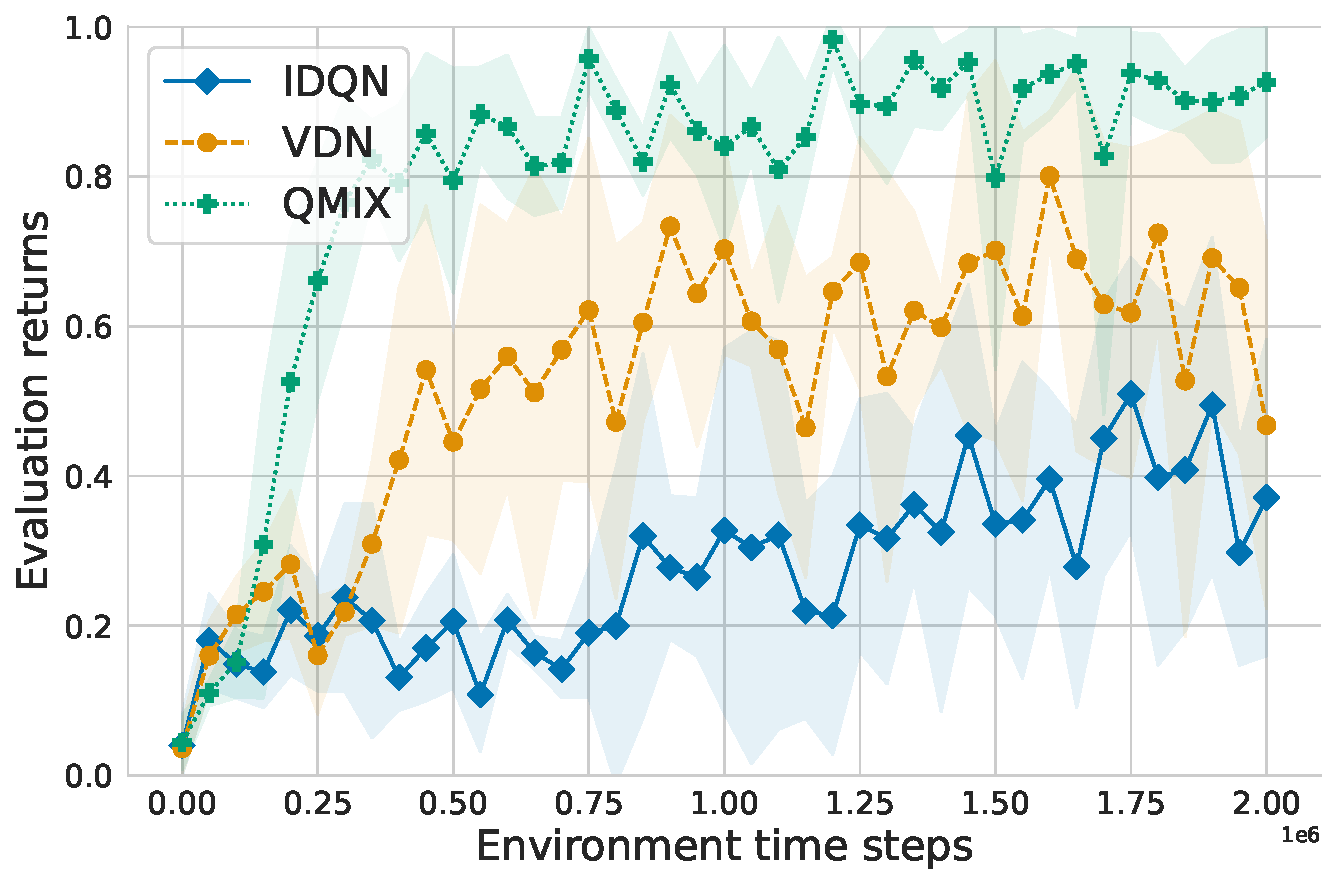
\includegraphics[width=.85\textwidth]{images/chapter_9/vd_lbf-8x8-2p-3f.pdf}
            \end{subfigure}
        }
    \end{figure}
\end{frame}

\begin{frame}{Summary}

\fat{We covered:}
    \blist
        \item Training and execution modes
        \item Independent learning with deep reinforcement learning
        \item Multi-agent policy gradient algorithms
        \item Value decomposition in common-reward games
    \elist

\fat{Next we'll cover:}

    \blist
        \item Agent modeling with deep learning
        \item Parameter and experience sharing
        \item Policy self-play in zero-sum games
        \item Population-based training
    \elist
    
\end{frame}

\end{document}
